\chapter{空间向量与立体几何}

本章介绍空间上的向量,对必修第六章(平面向量)的拓展,大致路数、重点和难点和第六章平面向量类似。

本章要点:
\begin{itemize}
    \item 空间向量及其几何意义。
\end{itemize}

\begin{tcolorbox}
自行对比第六章的目录,看看结构是不是高度相似。
\end{tcolorbox}

\begin{tcolorbox}
大学数学中关于三维空间的向量问题在微积分和线性代数中讲述,特别是线性代数,一整本书都在讲述向量。对比之下,高中课本的49页篇幅实在过于粗浅,加之向量接触时间短,所以需要反复仔细阅读课本,深刻领会。
\end{tcolorbox}

\newpage
\section{空间向量及其运算}

本节要点:
\begin{itemize}
    \item 掌握向量的概念;
    \item 掌握向量运算的概念及其法则;
    \item 深刻理解向量运算的几何意义。
\end{itemize}

%============================================================
\subsection{空间向量及其线性运算}

\begin{definition}
我们称空间内既有大小又有方向的量为{\bf 向量},常用粗体小写记作$\boldsymbol{a},\boldsymbol{b},\boldsymbol{c}$,同时称向量的大小为{\bf 长度}或{\bf 模}。若$\left| \boldsymbol{a} \right|=0$,称为{\bf 零向量},记作$\mathbf{0}$;若$\left| \boldsymbol{a} \right|=1$,称为{\bf 单位向量}。若数个向量的方向一致或反向,则称它们为{\bf 共线向量}或{\bf 平行向量};若数个向量平行于同一个平面,则称它们为{\bf 共面向量},显然任意两个向量必共面。
\end{definition}

\begin{tcolorbox}
注意,向量的定义中并没有规定起点。
\end{tcolorbox}

几何上,向量的加法满足平行六面体法则,向量的数乘表示伸缩,且有如下运算法则:
\begin{align*}
&\boldsymbol{a}+\boldsymbol{b}=\boldsymbol{b}+\boldsymbol{a} \\
&\left( \boldsymbol{a}+\boldsymbol{b} \right) +\boldsymbol{c}=\boldsymbol{a}+\left( \boldsymbol{b}+\boldsymbol{c} \right) \\
&\lambda \left( \mu \boldsymbol{a} \right) =\left( \lambda \mu \right) \boldsymbol{a} \\
&\left( \lambda +\mu \right) \boldsymbol{a}=\lambda \boldsymbol{a}+\mu \boldsymbol{a} \\
&\lambda \left( \boldsymbol{a}+\boldsymbol{b} \right) =\lambda \boldsymbol{a}+\lambda \boldsymbol{b}
\end{align*}

\begin{theorem}
不难得到以下两个定理:
\begin{itemize}
    \item 平行定理:$\boldsymbol{a}\parallel \boldsymbol{b}\Leftrightarrow \boldsymbol{a}=\lambda \boldsymbol{b}$
    \item 共面定理:$\boldsymbol{p}\text{与}\boldsymbol{a},\boldsymbol{b}\text{共面}\Leftrightarrow \boldsymbol{p}=x\boldsymbol{a}+y\boldsymbol{b}$
\end{itemize}
\end{theorem}

%============================================================
\subsection{空间向量的数量积运算}

\begin{definition}[数量积]
设$\boldsymbol{a},\boldsymbol{b}$为两个空间向量,我们称它们各自的模的乘积和它们的夹角的余弦的乘积为它们的{\bf 数量积},也称{\bf 内积},记作$\boldsymbol{a}\cdot \boldsymbol{b}$,即:
\[
\boldsymbol{a}\cdot \boldsymbol{b}:=\left| \boldsymbol{a} \right|\left| \boldsymbol{b} \right|\cos \theta
\]
\end{definition}

几何上,内积表示一向量在另一向量上的投影的乘积,有交换律和分配律,如下:
\begin{align*}
&\boldsymbol{a}\cdot \boldsymbol{b}=\boldsymbol{b}\cdot \boldsymbol{a} \\
&\boldsymbol{a}\cdot \left( \boldsymbol{b}+\boldsymbol{c} \right) =\boldsymbol{a}\cdot \boldsymbol{b}+\boldsymbol{a}\cdot \boldsymbol{c}
\end{align*}

\begin{tcolorbox}
注意,内积没有结合律。
\end{tcolorbox}

\begin{theorem}
不难得到以下三个定理:
\begin{itemize}
    \item 垂直定理:$\boldsymbol{a}\bot \boldsymbol{b}\Leftrightarrow \boldsymbol{a}\cdot \boldsymbol{b}=0$
    \item 模长定理:$\boldsymbol{a}\cdot \boldsymbol{a}=\left| \boldsymbol{a} \right|^2$
    \item 平行定理:$\boldsymbol{a}=\lambda _1\boldsymbol{b}_1+\lambda _2\boldsymbol{b}_2\Leftrightarrow \boldsymbol{a}\text{平行于}\boldsymbol{b}_1,\boldsymbol{b}_2\text{构成的平面}$
\end{itemize}
\end{theorem}

\begin{theorem}
使用内积不难证明以下两个重要的不等式:
\begin{itemize}
    \item 三角不等式:$\left| \boldsymbol{a}+\boldsymbol{b} \right|\leqslant \left| \boldsymbol{a} \right|+\left| \boldsymbol{b} \right|$,当且仅当$\boldsymbol{a},\boldsymbol{b}$同向时等号成立;
    \item 柯西—施瓦茨不等式:$\left| \boldsymbol{a}\cdot \boldsymbol{b} \right|\leqslant \left| \boldsymbol{a} \right|\cdot \left| \boldsymbol{b} \right|$,当且仅当$\boldsymbol{a},\boldsymbol{b}$平行时等号成立。
\end{itemize}
\end{theorem}

\begin{proof}
简单证明第一个不等式:
\begin{align*}
&\because \left| \boldsymbol{a}+\boldsymbol{b} \right|^2=\left( \boldsymbol{a}+\boldsymbol{b} \right) \cdot \left( \boldsymbol{a}+\boldsymbol{b} \right) =\boldsymbol{a}\cdot \boldsymbol{a}+2\left( \boldsymbol{a}\cdot \boldsymbol{b} \right) +\boldsymbol{b}\cdot \boldsymbol{b} \\
&\because \left( \left| \boldsymbol{a} \right|+\left| \boldsymbol{b} \right| \right) ^2=\left| \boldsymbol{a} \right|^2+2\left| \boldsymbol{a} \right|\left| \boldsymbol{b} \right|+\left| \boldsymbol{b} \right|^2 \\
&\because \boldsymbol{a}\cdot \boldsymbol{b}=\left| \boldsymbol{a} \right|\left| \boldsymbol{b} \right|\cos \theta \\
&\therefore \left| \boldsymbol{a}+\boldsymbol{b} \right|^2\leqslant \left( \left| \boldsymbol{a} \right|+\left| \boldsymbol{b} \right| \right) ^2
\end{align*}
\end{proof}

\begin{tcolorbox}
三角不等式表示的是加法,柯西—施瓦茨不等式表达的是乘法,两者反映了线性赋范空间上的守恒,XML。
\end{tcolorbox}

\begin{tcolorbox}
1.1.2中讨论空间向量内积的几何意义,我们将两个空间向量挪到一个平面内,用平面向量的内积解释空间向量,这反映了人类拓展知识的方法,即用已有的知识拓展研究未知并获得新的知识。

例3很有意思,仔细体会,例题如何从定义出发用代数的方法证明,例题并没有用纯几何的方法。
\end{tcolorbox}

%============================================================
\subsection{拓展讨论:向量外积}

两个向量还有外积,定义略,我看外积的模:
\[
\left| \boldsymbol{a}\times \boldsymbol{b} \right|=\left| \boldsymbol{a} \right|\left| \boldsymbol{b} \right|\sin \theta
\]
表示$\boldsymbol{a},\boldsymbol{b}$构成的平行四边形的面积,和内积有关系:
\[
\left| \boldsymbol{a}\times \boldsymbol{b} \right|^2+\left( \boldsymbol{a}\cdot \boldsymbol{b} \right) ^2=\left| \boldsymbol{a} \right|\left| \boldsymbol{b} \right|
\]

%============================================================
\subsection{习题}

\begin{example}[综合运用7,难度$\star $]
如图,正方体$ABCD-A'B'C'D'$的棱长为$a$。
\begin{enumerate}
    \item 求$A'B$和$B'C$的夹角;
    \item 求证:$A'B\bot AC'$。
\end{enumerate}
\end{example}

\begin{figure}[h]
\centering
\begin{tikzpicture}[style={x={(-155:0.5)},y={(1cm,0)},z={(0,1cm)}}, line join=round, scale=2]
\mydrawcube{A}{B}{C}{D}{A'}{B'}{C'}{D'}
\draw[thick,blue] (A')--(B) (B')--(C);
\draw[dashed,blue] (A)--(C');
\draw[thick,red] (D')--(B');
\draw[dashed,red] (D')--(C);
\end{tikzpicture}
\end{figure}

解一,向量法:

(1)
\[
\cos \theta =\frac{\overrightarrow{A'B}\cdot \overrightarrow{B'C}}{\left| \overrightarrow{A'B} \right|\cdot \left| \overrightarrow{B'C} \right|}=\frac{\left( \overrightarrow{AB}-\overrightarrow{AA'} \right) \cdot \left( \overrightarrow{BC}-\overrightarrow{BB'} \right)}{\left| \overrightarrow{A'B} \right|\cdot \left| \overrightarrow{B'C} \right|}=\frac{\overrightarrow{AA'}\cdot \overrightarrow{BB'}}{\sqrt{2}a\cdot \sqrt{2}a}=\frac{1}{2}
\]

(2)
\[
\overrightarrow{A'B}\cdot \overrightarrow{AC'}=\left( \overrightarrow{AB}-\overrightarrow{AA'} \right) \cdot \left( \overrightarrow{AB}+\overrightarrow{AD}+\overrightarrow{CC'} \right) =a^2-a^2=0
\]

解二,几何法:

(1)可以用纯几何的方法,$A'B$和$B'C$的夹角也即$D'C$和$B'C$的夹角,添加如图红色辅助线,不难发现$\bigtriangleup D'B'C$为等边三角形,后略。

深入分析:

我可以试着分析若要$A'B\bot AC'$,则该几何体需要满足的条件。
\begin{align*}
&\overrightarrow{A'B}\cdot \overrightarrow{AC'}=\left( \overrightarrow{AB}-\overrightarrow{AA'} \right) \cdot \left( \overrightarrow{AB}+\overrightarrow{AD}+\overrightarrow{CC'} \right) \\
&=\overrightarrow{AB}\cdot \overrightarrow{AB}-\overrightarrow{AA'}\cdot \overrightarrow{AB}+\overrightarrow{AB}\cdot \overrightarrow{AD}-\overrightarrow{AA'}\cdot \overrightarrow{AD}+\overrightarrow{AB}\cdot \overrightarrow{CC'}-\overrightarrow{AA'}\cdot \overrightarrow{CC'}
\end{align*}
当对棱平行且等长时:
\begin{align*}
&=-\overrightarrow{AA'}\cdot \overrightarrow{AB}+\overrightarrow{AB}\cdot \overrightarrow{AD}-\overrightarrow{AA'}\cdot \overrightarrow{AD}+\overrightarrow{AB}\cdot \overrightarrow{CC'} \\
&=\overrightarrow{AB}\cdot \left( \overrightarrow{AD}-\overrightarrow{AA'} \right) +\overrightarrow{AA'}\cdot \left( \overrightarrow{AB}-\overrightarrow{AD} \right) \\
&=\overrightarrow{AB}\cdot \overrightarrow{A'D}+\overrightarrow{AA'}\cdot \overrightarrow{DB}
\end{align*}
侧面均为菱形。

\begin{tcolorbox}
本题考察向量内积的几何意义。
\end{tcolorbox}

~

\begin{example}[拓广探索9,难度:$\star $]
如图,在四面体$OABC$中,$OA\bot BC$,$OB\bot AC$。求证:$OC\bot AB$。
\end{example}

\begin{figure}[h]
\centering
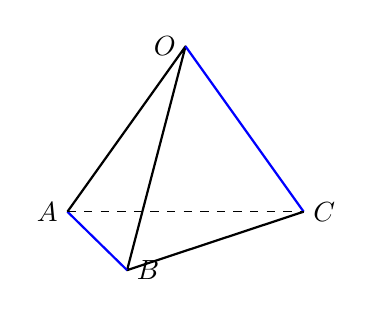
\begin{tikzpicture}[style={x={(-135:0.5)},y={(1cm,0)},z={(0,1cm)}}, line join=round, scale=3]
\coordinate[label=left: {$A$}] (A) at (0,-0.5,0);
\coordinate[label=right:{$B$}] (B) at (0.7,0,0);
\coordinate[label=right:{$C$}] (C) at (0,0.5,0);
\coordinate[label=left: {$O$}] (O) at (0,0,0.7);
\draw[thick] (A)--(O)--(B)--(C);
\draw[thick,blue] (A)--(B) (O)--(C);
\draw[dashed] (A)--(C);
\end{tikzpicture}
\end{figure}

解:
\begin{align*}
\overrightarrow{OC}\cdot \overrightarrow{AB}&=\left( \overrightarrow{AC}-\overrightarrow{AO} \right) \cdot \left( \overrightarrow{CB}-\overrightarrow{CA} \right) \\
&=\overrightarrow{AC}\cdot \overrightarrow{CB}-\overrightarrow{AO}\cdot \overrightarrow{CB}-\overrightarrow{AC}\cdot \overrightarrow{CA}+\overrightarrow{AO}\cdot \overrightarrow{CA} \\
&=\overrightarrow{AC}\cdot \overrightarrow{CB}+\overrightarrow{AC}\cdot \overrightarrow{AC}+\overrightarrow{AO}\cdot \overrightarrow{CA} \\
&=\overrightarrow{AC}\cdot \overrightarrow{AB}-\overrightarrow{AO}\cdot \overrightarrow{AC} \\
&=\overrightarrow{AC}\cdot \overrightarrow{OB}=0
\end{align*}

深入分析:

我们证明了在任意的四面体中,只要两组对棱垂直,则第三组对棱一定垂直。我们可以进一步分析,这样三组对棱垂直的情况下,四面体会有什么性质。

以$OB\bot AC$为例,意思就是$B,O$两点在$AC$上的投影重合,也即任意两个顶点在对面棱上的投影重合。根据这个结论建立如下左图的坐标系,可得:
\begin{align*}
&\because \begin{cases}
	OA\bot BC\Rightarrow \left( 0,y_A,-z_O \right) \cdot \left( -x_B,y_C,-z_B \right) =0\\
	OC\bot BA\Rightarrow \left( 0,y_C,-z_O \right) \cdot \left( -x_B,y_A,-z_B \right) =0\\
\end{cases} \\
&\therefore y_Ay_C+z_Oz_B=0
\end{align*}
四面体不一定非要正四面体,特别地,当$z_B=0$时,要么$y_A=0$要么$y_C=0$,四面体为长方体的一个角,如下右图。

\begin{figure}[h]
\centering
\begin{minipage}{.49\textwidth}
\centering
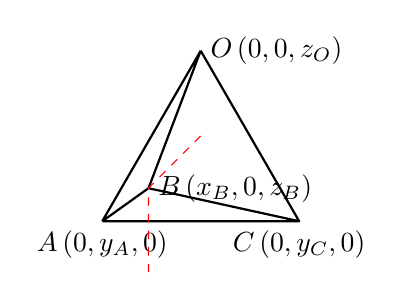
\begin{tikzpicture}[style={x={(-135:0.5)},y={(1cm,0)},z={(0,1cm)}}, line join=round, scale=2.5]
\mydrawxyz{0}{1.1}{-0.8}{0.8}{0}{1.1}
\coordinate[label=below:{$A\left( 0,y_A,0 \right) $}]   (A) at (0,-0.5,0);
\coordinate[label=below:{$C\left( 0,y_C,0 \right) $}]   (C) at (0,0.5,0);
\coordinate[label=right:{$B\left( x_B,0,z_B \right) $}] (B) at (0.75,0,0.433);
\coordinate[label=right:{$O\left( 0,0,z_O \right) $}]   (O) at (0,0,0.866);
\coordinate (Bx) at (0.75,0,0);
\coordinate (Bz) at (0,0,0.433);
\draw[thick] (O)--(A) (O)--(B) (O)--(C) (A)--(B)--(C)--(A);
\draw[dashed,red] (Bz)--(B)--(Bx);
\end{tikzpicture}
\end{minipage}
\begin{minipage}{.49\textwidth}
\centering
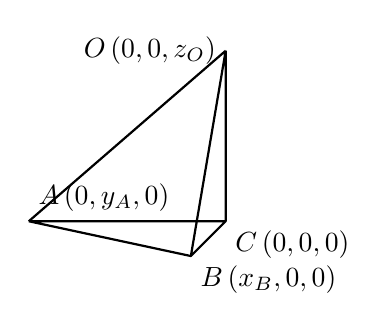
\begin{tikzpicture}[style={x={(-135:0.5)},y={(1cm,0)},z={(0,1cm)}}, line join=round, scale=2.5]
\mydrawxyz{0}{1.1}{-1.3}{0.3}{0}{1.1}
\coordinate[label=above right:{$A\left( 0,y_A,0 \right) $}] (A) at (0,-1,0);
\coordinate[label=below right:{$C\left( 0,0,0 \right) $}]   (C) at (0,0,0);
\coordinate[label=below right:{$B\left( x_B,0,0 \right) $}] (B) at (0.5,0,0);
\coordinate[label=left:       {$O\left( 0,0,z_O \right) $}] (O) at (0,0,0.866);
\draw[thick] (O)--(A) (O)--(B) (O)--(C) (A)--(B)--(C)--(A);
\end{tikzpicture}
\end{minipage}
\end{figure}

\begin{tcolorbox}
本题依然考察向量内积的几何意义。
\end{tcolorbox}

~

\begin{example}[拓广探索10,难度:$\star \star $]
如图,在四面体$OABC$中,$OA=OB,CA=CB$,$E,F,G,H$分别是$OA,OB,BC,CA$的中点。求证:四边形$EFGH$是矩形。
\end{example}

\begin{figure}[h]
\centering
\begin{tikzpicture}[style={x={(-160:0.7)},y={(1cm,-0.2cm)},z={(0,1cm)}}, line join=round, scale=2.5]
\coordinate[label=above:      {$A$}] (A) at (-0.5,-0.3,0);
\coordinate[label=left:       {$B$}] (B) at (0.5,-0.3,0);
\coordinate[label=right:      {$C$}] (C) at (0,1,0);
\coordinate[label=above:      {$O$}] (O) at (0,0,1);
\coordinate[label=left:       {$F$}] (F) at ($(O)!0.5!(B)$);
\coordinate[label=above:      {$E$}] (E) at ($(O)!0.5!(A)$);
\coordinate[label=below:      {$G$}] (G) at ($(C)!0.5!(B)$);
\coordinate[label=right:      {$H$}] (H) at ($(C)!0.5!(A)$);
\coordinate[label=above left: {$D$}] (D) at ($(A)!0.5!(B)$);
\coordinate[label=above:      {$M$}] (M) at ($(F)!0.5!(E)$);
\coordinate[label=below right:{$N$}] (N) at ($(G)!0.5!(H)$);
\draw[thick] (O)--(B)--(C)--(O);
\draw[dashed] (A)--(O) (A)--(B) (A)--(C);
\draw[thick,blue] (F)--(G);
\draw[dashed,blue] (F)--(E)--(H)--(G);
\fill[blue!50!white,opacity=0.5] (F)--(G)--(H)--(E)--cycle;
\draw[dashed,red] (O)--(D)--(C) (M)--(N);
\end{tikzpicture}
\end{figure}

解:

首先,不难通过$\overrightarrow{FG}=\overrightarrow{EH}$证明四边形$EFGH$是平行四边形。

再证明$\angle EFG$为直角。直接用向量的方法证明$\overrightarrow{FG}\cdot \overrightarrow{FE}=0$较复杂。找到$AB$中点$D$,连接$OD,CD$,不难证明$OD,CD$是三角形的中垂线,而且$FG,MN$平行且相等,所以也即证明$\overrightarrow{MN}\cdot \overrightarrow{FE}=0$。
\[
\overrightarrow{MN}\cdot \overrightarrow{FE}=\left( \overrightarrow{DN}-\overrightarrow{DM} \right) \cdot \overrightarrow{FE}=\overrightarrow{DN}\cdot \overrightarrow{GH}-\overrightarrow{DM}\cdot \overrightarrow{FE}
\]

深入分析:

不难发现,当$AB$长度一定时,$OD,CD$决定了矩形面积,我们可以考察一下当矩形面积$S$和$DO,DC$长度的关系。
\begin{align*}
&\because S=\frac{AB}{2}\cdot \frac{OC}{2} \\
&\because \cos \angle ODC=\frac{DO^2+DC^2-OC^2}{2\cdot DO\cdot DC} \\
&\therefore S=\frac{AB}{4}\cdot \left( DO^2+DC^2-2\cos \angle ODC\cdot DO\cdot DC \right)
\end{align*}
易得:
\begin{itemize}
    \item 当$S$恒定时,$OD,CD$是一个椭圆关系,可设$\angle ODC\in \left( 0,\frac{\pi}{2} \right] $,则$2\cos \angle ODC\in \left[ 0,2 \right) $,椭圆转了45°,特别地,当$DO\bot DC$时,为圆;
    \item 当$OD,CD$相互制约时,$S$有最值。
\end{itemize}

\begin{tcolorbox}
本题需要添加辅助线,用纯几何+向量的方法,事半功倍。
\end{tcolorbox}






\newpage
\section{空间向量基本定理}

本节要点:
\begin{itemize}
    \item 掌握空间向量基本定理。
\end{itemize}

\begin{theorem}[空间向量基本定理]
设$\boldsymbol{a},\boldsymbol{b},\boldsymbol{c}$为三个不共面的空间向量,则对于任意向量$\boldsymbol{p}$,存在唯一的有序实数组$\left( x,y,z \right) $,使得
\[
\boldsymbol{p}=x\boldsymbol{a}+y\boldsymbol{b}+z\boldsymbol{c}
\]
我们把$\left\{ \boldsymbol{a},\boldsymbol{b},\boldsymbol{c} \right\} $称作空间的一个{\bf 基},把$\boldsymbol{a},\boldsymbol{b},\boldsymbol{c}$称作{\bf 基向量},对应的$\left( x,y,z \right) $称为$\boldsymbol{p}$在该组基下的{\bf 坐标}。
\end{theorem}

该定理和平面向量基本定理一样,指的是向量可以由基组合得到。也要注意,定理表达的意思是给定一个基就有一个坐标与之对应,所以不同的基有不同的坐标,但$\boldsymbol{p}$还是那个$\boldsymbol{p}$,也即:
\[
\boldsymbol{p}=x\boldsymbol{a}+y\boldsymbol{b}+z\boldsymbol{c}=l\boldsymbol{d}+m\boldsymbol{e}+n\boldsymbol{f}
\]

%============================================================
\subsection{习题}

\begin{example}[拓广探索8,难度:$\star \star $]
已知四面体中三组相对棱的中点间的距离都相等,求证:这个四面体相对的棱两两垂直。
\end{example}

解:

如下图,不难得到三组相对棱的中点连接的向量:

\begin{figure}[h]
\centering
\begin{minipage}{.32\textwidth}
\centering
\begin{tikzpicture}[style={x={(-135:0.5)},y={(1cm,0)},z={(0,1cm)}}, line join=round, scale=2.5]
\coordinate[label=left:      {$A$}] (A) at (0,-0.5,0);
\coordinate[label=below:     {$B$}] (B) at (0.7,0,0);
\coordinate[label=right:     {$C$}] (C) at (0,0.5,0);
\coordinate[label=above:     {$O$}] (O) at (0,0,0.7);
\coordinate[label=below left:{$D$}] (D) at ($(A)!0.5!(B)$);
\coordinate[label=right:     {$E$}] (E) at ($(O)!0.5!(C)$);
\draw[thick] (B)--(O)--(A)--(B)--(C)--(O);
\draw[dashed] (A)--(C);
\draw[dashed,red] (D)--(E) (O)--(D)--(C);
\end{tikzpicture}
\end{minipage}
\begin{minipage}{.32\textwidth}
\centering
\begin{tikzpicture}[style={x={(-135:0.5)},y={(1cm,0)},z={(0,1cm)}}, line join=round, scale=2.5]
\coordinate[label=left:       {$A$}]  (A) at (0,-0.5,0);
\coordinate[label=below:      {$B$}]  (B) at (0.7,0,0);
\coordinate[label=right:      {$C$}]  (C) at (0,0.5,0);
\coordinate[label=above:      {$O$}]  (O) at (0,0,0.7);
\coordinate[label=below right:{$D'$}] (D) at ($(A)!0.5!(C)$);
\coordinate[label=left:       {$E'$}] (E) at ($(O)!0.5!(B)$);
\draw[thick] (B)--(O)--(A)--(B)--(C)--(O);
\draw[dashed] (A)--(C);
\draw[dashed,red] (D)--(E) (O)--(D)--(B);
\end{tikzpicture}
\end{minipage}
\begin{minipage}{.32\textwidth}
\centering
\begin{tikzpicture}[style={x={(-135:0.5)},y={(1cm,0)},z={(0,1cm)}}, line join=round, scale=2.5]
\coordinate[label=left:       {$A$}]   (A) at (0,-0.5,0);
\coordinate[label=below:      {$B$}]   (B) at (0.7,0,0);
\coordinate[label=right:      {$C$}]   (C) at (0,0.5,0);
\coordinate[label=above:      {$O$}]   (O) at (0,0,0.7);
\coordinate[label=below right:{$D''$}] (D) at ($(B)!0.5!(C)$);
\coordinate[label=left:       {$E''$}] (E) at ($(O)!0.5!(A)$);
\draw[thick] (B)--(O)--(A)--(B)--(C)--(O);
\draw[dashed] (A)--(C);
\draw[dashed,red] (D)--(E) (O)--(D)--(A);
\end{tikzpicture}
\end{minipage}
\end{figure}

\begin{align*}
&\overrightarrow{DE}=-\frac{1}{4}\left( \overrightarrow{OB}+\overrightarrow{OA}+\overrightarrow{CB}+\overrightarrow{CA} \right) \\
&\overrightarrow{D'E'}=-\frac{1}{4}\left( \overrightarrow{OA}+\overrightarrow{OC}+\overrightarrow{BA}+\overrightarrow{BC} \right) \\
&\overrightarrow{D''E''}=-\frac{1}{4}\left( \overrightarrow{AB}+\overrightarrow{AC}+\overrightarrow{OB}+\overrightarrow{OC} \right)
\end{align*}
若要平方进行长度相等,非常复杂,我们简化,使之都用$OX$表示:
\begin{align*}
&\overrightarrow{DE}=-\frac{1}{2}\left( \overrightarrow{OB}+\overrightarrow{OA}-\overrightarrow{OC} \right) \\
&\overrightarrow{D'E'}=-\frac{1}{2}\left( \overrightarrow{OA}+\overrightarrow{OC}-\overrightarrow{OB} \right) \\
&\overrightarrow{D''E''}=-\frac{1}{2}\left( \overrightarrow{OB}+\overrightarrow{OC}-\overrightarrow{OA} \right)
\end{align*}
取$\left| \overrightarrow{DE} \right|=\left| \overrightarrow{D'E'} \right|$分析:
\begin{align*}
&\because \left| \overrightarrow{DE} \right|=\left| \overrightarrow{D'E'} \right| \\
&\therefore \left( \overrightarrow{OB}+\overrightarrow{OA}-\overrightarrow{OC} \right) ^2=\left( \overrightarrow{OA}+\overrightarrow{OC}-\overrightarrow{OB} \right) ^2 \\
&\therefore \overrightarrow{OB}\cdot \overrightarrow{OA}-\overrightarrow{OA}\cdot \overrightarrow{OC}=\overrightarrow{OA}\cdot \overrightarrow{OC}-\overrightarrow{OA}\cdot \overrightarrow{OB} \\
&\therefore \overrightarrow{OB}\cdot \overrightarrow{OA}-\overrightarrow{OA}\cdot \overrightarrow{OC}=0 \\
&\therefore \overrightarrow{OA}\cdot \left( \overrightarrow{OB}-\overrightarrow{OC} \right) =0 \\
&\therefore \overrightarrow{OA}\cdot \overrightarrow{CB}=0
\end{align*}
余下略。

深入分析:

结合上一节的拓广探索9,若三对棱垂直了,计算一下对棱的中点距。

\begin{figure}[h]
\centering
\begin{minipage}{.49\textwidth}
\centering
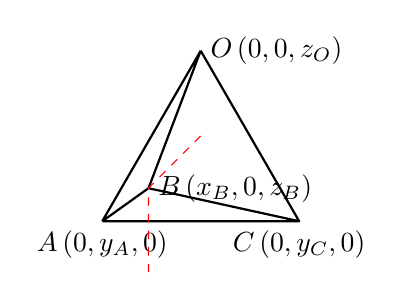
\begin{tikzpicture}[style={x={(-135:0.5)},y={(1cm,0)},z={(0,1cm)}}, line join=round, scale=2.5]
\mydrawxyz{0}{1.1}{-0.8}{0.8}{0}{1.1}
\coordinate[label=below:{$A\left( 0,y_A,0 \right) $}]   (A) at (0,-0.5,0);
\coordinate[label=below:{$C\left( 0,y_C,0 \right) $}]   (C) at (0,0.5,0);
\coordinate[label=right:{$B\left( x_B,0,z_B \right) $}] (B) at (0.75,0,0.433);
\coordinate[label=right:{$O\left( 0,0,z_O \right) $}]   (O) at (0,0,0.866);
\coordinate (Bx) at (0.75,0,0);
\coordinate (Bz) at (0,0,0.433);
\draw[thick] (O)--(A) (O)--(B) (O)--(C) (A)--(B)--(C)--(A);
\draw[dashed,red] (Bz)--(B)--(Bx);
\end{tikzpicture}
\end{minipage}
\begin{minipage}{.49\textwidth}
\centering
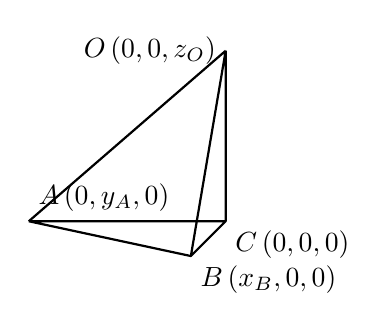
\begin{tikzpicture}[style={x={(-135:0.5)},y={(1cm,0)},z={(0,1cm)}}, line join=round, scale=2.5]
\mydrawxyz{0}{1.1}{-1.3}{0.3}{0}{1.1}
\coordinate[label=above right:{$A\left( 0,y_A,0 \right) $}] (A) at (0,-1,0);
\coordinate[label=below right:{$C\left( 0,0,0 \right) $}]   (C) at (0,0,0);
\coordinate[label=below right:{$B\left( x_B,0,0 \right) $}] (B) at (0.5,0,0);
\coordinate[label=left:       {$O\left( 0,0,z_O \right) $}] (O) at (0,0,0.866);
\draw[thick] (O)--(A) (O)--(B) (O)--(C) (A)--(B)--(C)--(A);
\end{tikzpicture}
\end{minipage}
\end{figure}

以$OA,BC$为例,它们的中点距为$\left( \frac{x_B}{2},\frac{y_A}{2},\frac{z_B}{2} \right) ,\left( 0,\frac{y_C}{2},\frac{z_O}{2} \right) $的距离,令$l$,则有:
\begin{align*}
&\because OA\bot BC\Rightarrow \left( 0,y_A,-z_O \right) \cdot \left( -x_B,y_C,-z_B \right) =0 \\
&\therefore y_Ay_C+z_Oz_B=0 \\
&\therefore l^2=\left( \frac{x_B}{2} \right) ^2+\left( \frac{y_A-y_C}{2} \right) ^2+\left( \frac{z_B-z_O}{2} \right) ^2 \\
&\therefore 4l^2={x_B}^2+{y_A}^2+{y_C}^2+{z_B}^2+{z_O}^2=OA^2+BC^2
\end{align*}
而且有:
\[
OA^2+BC^2=OC^2+AB^2=OB^2+AC^2
\]
这也是对棱垂直的四面体的性质,不难发现,正四面体和长方体一角都是该式的特殊形式。

\begin{tcolorbox}
本题思路简单,从定义出发,但是计算量大,如果不将一开始的表达式化简,几乎无解。
\end{tcolorbox}






\newpage
\section{空间向量及其运算的坐标表示}

本节要点:
\begin{itemize}
    \item 掌握向量运算的坐标表示。
\end{itemize}

%============================================================
\subsection{空间直角坐标系}

和平面向量一样,当我们定义了空间直角坐标系后,可以得到空间向量的3个等价表示方法:
\begin{itemize}
    \item $\overrightarrow{AB}$:表示三维空间的有向线段;
    \item $x\boldsymbol{i}+y\boldsymbol{j}+z\boldsymbol{k}$:表示{\it xyz}坐标系中的有向线段;
    \item $\left( x,y,z \right) $:表示{\it xyz}坐标系中的点。
\end{itemize}

\begin{tcolorbox}
这里要注意一点,直角坐标系的右手性是人为规定的。
\end{tcolorbox}

%============================================================
\subsection{空间向量运算的坐标系表示}

加法、数乘、内积的坐标表示如下:
\begin{align*}
&\boldsymbol{a}+\boldsymbol{b}=\left( x_{\boldsymbol{a}}+x_{\boldsymbol{b}} \right) \boldsymbol{i}+\left( y_{\boldsymbol{a}}+y_{\boldsymbol{b}} \right) \boldsymbol{j}+\left( z_{\boldsymbol{a}}+z_{\boldsymbol{b}} \right) \boldsymbol{k} \\
&\lambda \boldsymbol{a}=\lambda x_{\boldsymbol{a}}\boldsymbol{i}+\lambda y_{\boldsymbol{a}}\boldsymbol{j}+\lambda z_{\boldsymbol{a}}\boldsymbol{k} \\
&\boldsymbol{a}\cdot \boldsymbol{b}=x_{\boldsymbol{a}}\cdot x_{\boldsymbol{b}}+y_{\boldsymbol{a}}\cdot y_{\boldsymbol{b}}+z_{\boldsymbol{a}}\cdot z_{\boldsymbol{b}}=\left| \boldsymbol{a} \right|\left| \boldsymbol{b} \right|\cos \alpha
\end{align*}

%============================================================
\subsection{习题}

\begin{example}[拓广探索9,难度:$\star \star $]
$\left\{ \boldsymbol{a},\boldsymbol{b},\boldsymbol{c} \right\} $是空间的一个单位正交基底,向量$\boldsymbol{p}=\boldsymbol{a}+2\boldsymbol{b}+3\boldsymbol{c}$,$\left\{ \boldsymbol{a}+\boldsymbol{b},\boldsymbol{a}-\boldsymbol{b},\boldsymbol{c} \right\} $是空间的另一个基底,用$\left\{ \boldsymbol{a}+\boldsymbol{b},\boldsymbol{a}-\boldsymbol{b},\boldsymbol{c} \right\} $表示向量$\boldsymbol{p}$。
\end{example}

解:

$\boldsymbol{p}$在新坐标系下可表示为:
\[
\boldsymbol{p}=x\left( \boldsymbol{a}+\boldsymbol{b} \right) +y\left( \boldsymbol{a}-\boldsymbol{b} \right) +z\boldsymbol{c}=\left( x+y \right) \boldsymbol{a}+\left( x-y \right) \boldsymbol{b}+z\boldsymbol{c}
\]
于是:
\begin{align*}
&\begin{cases}
	x+y=1\\
	x-y=2\\
	z=3\\
\end{cases}\Rightarrow \begin{cases}
	x=\frac{3}{2}\\
	y=-\frac{1}{2}\\
	z=3\\
\end{cases} \\
&\boldsymbol{p}=\frac{3}{2}\left( \boldsymbol{a}+\boldsymbol{b} \right) -\frac{1}{2}\left( \boldsymbol{a}-\boldsymbol{b} \right) +3\boldsymbol{c}
\end{align*}

\begin{tcolorbox}
本题其实是对空间向量基本定理的拓展,任意向量在不同基下有不同的表示,但向量还是那个向量。
\end{tcolorbox}






\newpage
\section{空间向量的应用}

本节要点:
\begin{itemize}
    \item 掌握空间点线面的方程;
    \item 熟练掌握使用向量判断空间点线面的关系。
\end{itemize}

%============================================================
\subsection{用空间向量研究直线、平面的位置关系}

首先定义点、线、面的向量表达式。

{\bf 空间中的点}

直接用向量或其坐标表示:
\[
\overrightarrow{OP} \qquad \boldsymbol{p} \qquad \left( x_{\boldsymbol{p}},y_{\boldsymbol{p}},z_{\boldsymbol{p}} \right)
\]

{\bf 空间中的直线}

直线的定义是和给定点$P_0$构成的向量与给定向量$\boldsymbol{n}$平行的所有点的集合,即:
\[
\overrightarrow{P_0P}=\lambda \boldsymbol{n} \quad \text{或} \quad \left( x-x_0,y-y_0,z-z_0 \right) =\lambda \left( A,B,C \right)
\]
展开后得空间直线方程:
\[
\frac{x-x_0}{A}=\frac{y-y_0}{B}=\frac{z-z_0}{C}
\]
其中:
\begin{itemize}
    \item $\boldsymbol{n}=\left( A,B,C \right) $:直线的方向;
    \item $\left( x_0,y_0,z_0 \right) $:直线上一点$P_0$的坐标。
\end{itemize}

{\bf 空间中的平面}

平面的定义是和给定点$P_0$构成的向量与给定向量$\boldsymbol{n}$垂直得所有点得集合,即:
\[
\overrightarrow{P_0P}\cdot \boldsymbol{n}=0 \quad \text{或} \quad A\left( x-x_0 \right) +B\left( y-y_0 \right) +C\left( z-z_0 \right) =0
\]
展开后得到空间平面的一般方程:
\[
Ax+By+Cz+D=0
\]
其中:
\begin{itemize}
    \item $\boldsymbol{n}=\left( A,B,C \right) $:平面的法线方向;
    \item $\left( x_0,y_0,z_0 \right) $:平面上一点$P_0$的坐标。
\end{itemize}
特别地,当平面和{\it xyz}轴分别交于$x_0,y_0,z_0$时,则可以写成截距式:
\[
\frac{x}{x_0}+\frac{y}{y_0}+\frac{z}{z_0}=0
\]

\begin{tcolorbox}
以上定义中,关键在于点和方向。点好理解,直线或平面上的点,直线的方向也好理解,面的方向是第一次碰到,我们取平面的法线的方向作为平面的方向。还要注意,高中阶段的方向,不分正反!
\end{tcolorbox}

\begin{theorem}
根据以上定义,我们不难得到直线和平面关系的判定定理:
\begin{itemize}
    \item 若$\boldsymbol{l}_1=\lambda \boldsymbol{l}_2$,则两直线$l_1,l_2$平行;
    \item 若$\boldsymbol{l}\cdot \boldsymbol{n}=0$,则直线$l$平面$\alpha $平行;
    \item 若$\boldsymbol{n}_{\alpha}=\lambda \boldsymbol{n}_{\beta}$,则两平面$\alpha ,\beta $平行;
    \item 若$\boldsymbol{l}_1\cdot \boldsymbol{l}_2=0$,则两直线$l_1,l_2$垂直;
    \item 若$\boldsymbol{l}=\lambda \boldsymbol{n}$,则直线$l$平面$\alpha $垂直;
    \item 若$\boldsymbol{n}_{\alpha}\cdot \boldsymbol{n}_{\beta}=0$,则两平面$\alpha ,\beta $垂直。
\end{itemize}
\end{theorem}

\begin{table}[h]
\centering
\begin{tabular}{ccc}
    \toprule
     & 平行 & 垂直\\
    \midrule
    线线$l_1,l_2$ & $\boldsymbol{l}_1=\lambda \boldsymbol{l}_2$ & $\boldsymbol{l}_1\cdot \boldsymbol{l}_2=0$\\
    线面$l,\alpha $ & $\boldsymbol{l}\cdot \boldsymbol{n}=0$ & $\boldsymbol{l}=\lambda \boldsymbol{n}$\\
    面面$\alpha ,\beta $ & $\boldsymbol{n}_{\alpha}=\lambda \boldsymbol{n}_{\beta}$ & $\boldsymbol{n}_{\alpha}\cdot \boldsymbol{n}_{\beta}=0$\\
    \bottomrule
\end{tabular}
\end{table}

%============================================================
\subsection{用空间向量研究距离、夹角问题}

如下图,点$P$到直线和平面的距离表达式:

\begin{figure}[h]
\centering
\begin{minipage}{.49\textwidth}
\centering
\begin{tikzpicture}[line join=round, scale=0.5]
\coordinate[label=below:{$A$}]                (A)  at (0,0);
\coordinate[label=below:{$Q$}]                (Q)  at (4,0);
\coordinate[label=right:{$P$}]                (P)  at (4,3);
\coordinate[label=right:{$\boldsymbol{l}_0$}] (l0) at (6,0);
\draw[thick] ($(A)!-0.5!(Q)$)--($(A)!1.5!(Q)$);
\draw[thick,-stealth] (A)--(P);
\draw[dashed] (Q)--(P);
\end{tikzpicture}
\end{minipage}
\begin{minipage}{.49\textwidth}
\centering
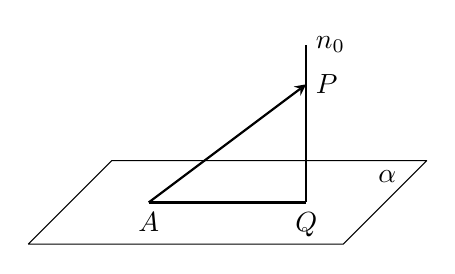
\begin{tikzpicture}[style={x={(-135:0.5)},y={(1cm,0)},z={(0,1cm)}}, line join=round, scale=0.5]
\draw (3,-2,0)--(3,6,0)--(-3,6,0)--(-3,-2,0)--(3,-2,0);
\coordinate[label=below:{$\alpha $}]          (a)  at (-3,5,0);
\coordinate[label=below:{$A$}]                (A)  at (0,0,0);
\coordinate[label=below:{$Q$}]                (Q)  at (0,4,0);
\coordinate[label=right:{$P$}]                (P)  at (0,4,3);
\coordinate[label=right:{$\boldsymbol{n}_0$}] (n0) at (0,4,4);
\draw[thick] (A)--(Q);
\draw[thick,-stealth] (A)--(P);
\draw[thick] (Q)--(n0);
\end{tikzpicture}
\end{minipage}
\end{figure}

\[
PQ=\sqrt{\overrightarrow{AP}^2-\left( \overrightarrow{AP}\cdot \boldsymbol{l}_0 \right) ^2} \qquad \qquad PQ=\left| \overrightarrow{AP}\cdot \boldsymbol{n}_0 \right|
\]
其中:
\begin{itemize}
    \item $\boldsymbol{l}_0$:直线的单位方向向量;
    \item $\boldsymbol{n}_0$:平面的单位法向方向向量。
\end{itemize}

~

如下图,线线、线面、面面夹角的余弦表达式:
\[
\cos \theta =\frac{\left| \boldsymbol{l}_1\cdot \boldsymbol{l}_2 \right|}{\left| \boldsymbol{l}_1 \right|\left| \boldsymbol{l}_2 \right|} \qquad \sin \theta =\frac{\left| \boldsymbol{l}\cdot \boldsymbol{n} \right|}{\left| \boldsymbol{l} \right|\left| \boldsymbol{n} \right|} \qquad \cos \theta =\frac{\left| \boldsymbol{n}_1\cdot \boldsymbol{n}_2 \right|}{\left| \boldsymbol{n}_1 \right|\left| \boldsymbol{n}_2 \right|}
\]

\begin{figure}[h]
\centering
\begin{minipage}{.32\textwidth}
\centering
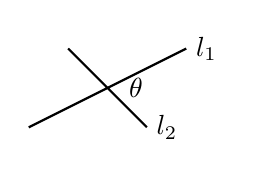
\begin{tikzpicture}[line join=round, scale=0.5]
\coordinate                                   (l11) at (-2,-1);
\coordinate[label=right:{$\boldsymbol{l}_1$}] (l12) at (2,1);
\coordinate                                   (l21) at (-1,1);
\coordinate[label=right:{$\boldsymbol{l}_2$}] (l22) at (1,-1);
\coordinate[label=right:{$\theta $}]          (t)   at (0.3,0);
\draw[thick] (l11)--(l12) (l21)--(l22);
\end{tikzpicture}
\end{minipage}
\begin{minipage}{.32\textwidth}
\centering
\begin{tikzpicture}[style={x={(-135:0.5)},y={(1cm,0)},z={(0,1cm)}}, line join=round, scale=0.3]
\draw (3,-2,0)--(3,6,0)--(-3,6,0)--(-3,-2,0)--(3,-2,0);
\coordinate                                       (A) at (0,0,0);
\coordinate                                       (Q) at (0,4,0);
\coordinate                                       (P) at (0,4,3);
\coordinate[label=above left: {$\boldsymbol{l}$}] (l) at ($(A)!0.5!(P)$);
\coordinate[label=right:      {$\boldsymbol{n}$}] (n) at (P);
\coordinate[label=above right:{$\theta $}]        (t) at (0,1,0);
\draw[thick] (A)--(Q);
\draw[thick,-stealth] (A)--(P);
\draw[thick,-stealth] (Q)--(P);
\end{tikzpicture}
\end{minipage}
\begin{minipage}{.32\textwidth}
\centering
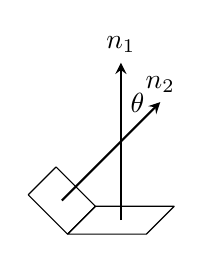
\begin{tikzpicture}[style={x={(-135:0.5)},y={(1cm,0)},z={(0,1cm)}}, line join=round, scale=0.5]
\draw (1,2,0)--(1,0,0)--(-1,0,0)--(-1,2,0)--(1,2,0);
\draw (1,0,0)--(1,-1,1)--(-1,-1,1)--(-1,0,0)--(1,0,0);
\coordinate[label=above:      {$\boldsymbol{n}_1$}] (n1) at (0,1,4);
\coordinate[label=above:      {$\boldsymbol{n}_2$}] (n2) at (0,2,3);
\coordinate[label=above right:{$\theta $}]          (t)  at (0,1,2.5);
\draw[thick,-stealth] (0,1,0)--(n1);
\draw[thick,-stealth] (0,-0.5,0.5)--(n2);
\end{tikzpicture}
\end{minipage}
\end{figure}

\begin{tcolorbox}
本节的例1、例2、例3、例9、例10,都值得反复阅读。
\end{tcolorbox}

%============================================================
\subsection{习题}

\begin{example}[拓广探索18,难度:$\star \star \star $]
在如图所示的实验装置中,两个正方形框架$ABCD$,$ABEF$的边长都是1,且它们所在的平面互相垂直。活动弹子$M,N$分别在正方形对角线$AC$和$BF$上移动,且$CM$和$BN$的长度保持相等,记$CM=BN=a,0<a<\sqrt{2}$。
\begin{enumerate}
    \item 求$MN$的长;
    \item $a$为何值时,$MN$的长最小?
    \item 当$MN$的长最小时,求平面$MNA$和$MNB$夹角的余弦值。
\end{enumerate}
\end{example}

\begin{figure}[h]
\centering
\begin{tikzpicture}[style={x={(-145:0.8)},y={(1cm,-0.2cm)},z={(0,1cm)}}, line join=round, scale=2]
\pgfmathparse{0.6/2}
\mydrawxyz{0}{1.4}{0}{1.4}{0}{1.4}
\coordinate[label=above right:{$B$}] (B) at (0,0,0);
\coordinate[label=below:      {$A$}] (A) at (1,0,0);
\coordinate[label=right:      {$C$}] (C) at (0,0,1);
\coordinate[label=left:       {$D$}] (D) at (1,0,1);
\coordinate[label=above:      {$E$}] (E) at (0,1,0);
\coordinate[label=below:      {$F$}] (F) at (1,1,0);
\coordinate[label=left:       {$M$}] (M) at ($(A)!0.5!(C)$);
\coordinate[label=right:      {$N$}] (N) at ($(B)!0.5!(F)$);
\coordinate[label=left:       {$a$}] (a) at ($(C)!0.5!(M)$);
\coordinate[label=right:      {$a$}] (a) at ($(B)!0.5!(N)$);
\draw[thick] (A)--(B)--(C)--(D)--(A)--(C) (F)--(B)--(E)--(F)--(A) (A)--(N) (B)--(M);
\draw[thick,blue] (M)--(N);
\fill (M) circle (\pgfmathresult mm);
\fill (N) circle (\pgfmathresult mm);
\fill[blue!50!white,opacity=0.5] (M)--(N)--(B)--cycle;
\fill[pink!50!white,opacity=0.5] (M)--(N)--(A)--cycle;
\end{tikzpicture}
\end{figure}

解:

(1)以$B$为原点建立直角坐标系。根据关系可得$M,N$坐标$M=\left( x,0,1-x \right) ,N=\left( x,x,0 \right) $,其中$\sqrt{2}x=a$,于是:
\[
MN=\sqrt{x^2+\left( 1-x \right) ^2}=\sqrt{2x^2-2x+1}=\sqrt{\left( \sqrt{2}x-\frac{1}{\sqrt{2}} \right) ^2+\frac{1}{2}}
\]

(2)可见,当$x=\frac{1}{2}$时,$MN$最小,为$\sqrt{\frac{1}{2}}$,此时$a=\frac{\sqrt{2}}{2}$。

(3)不难发现$\bigtriangleup AMN,\bigtriangleup BMN$均为等边三角形,后略。

深入分析:

探讨一下$MN$最值。首先有一个直觉,高中阶段的不等值最终都可以归结为基本不等式,$MN$两头都是$CB=AF=1$,一定是对称点取到最值,事实也是如此。另一个直觉,异面直线距离最短,$MN$应该是距离,但显然结果的$MN$并不是距离,这点从$MN$和$AC,BF$都不垂直可以得出。两个直觉发生矛盾了。

假设$M,N$各自运动,我们看看什么时候$MN$最短。
另$M,N$坐标$M=\left( x_m,0,1-x_m \right) ,N=\left( x_n,x_n,0 \right) $,于是:
\begin{align*}
MN&=\sqrt{\left( x_m-x_n \right) ^2+{x_n}^2+\left( 1-x_m \right) ^2} \\
&=\sqrt{2{x_m}^2-2x_mx_n+2{x_n}^2+1-2x_m}
\end{align*}
另$y=2{x_m}^2-2x_mx_n+2{x_n}^2+1-2x_m$,计算一阶和二阶偏导:
\begin{align*}
&\because \begin{cases}
	\frac{\partial y}{\partial x_m}=4x_m-2x_n-2=0\\
	\frac{\partial y}{\partial x_n}=-2x_m+4x_n=0\\
\end{cases} \quad \begin{cases}
	A=\frac{\partial ^2y}{{\partial x_m}^2}=4\\
	C=\frac{\partial ^2y}{{\partial x_n}^2}=4\\
	B=\frac{\partial ^2y}{\partial x_m\partial x_n}=-2\\
\end{cases} \\
&\therefore x_m=\frac{2}{3},x_n=\frac{1}{3}
\end{align*}
由于$AC>B,A>0$,所以该值为最小值,此时:
\begin{align*}
&M=\left( \frac{2}{3},0,\frac{1}{3} \right) ,N=\left( \frac{1}{3},\frac{1}{3},0 \right) \\
&MN=\sqrt{\left( 1/3 \right) ^2+\left( 1/3 \right) ^2+\left( 1/3 \right) ^2}=1/\sqrt{3}
\end{align*}
再考察$\bigtriangleup AMN$:
\begin{align*}
&A=\left( 1,0,0 \right) \\
&AM=\sqrt{\left( 1/3 \right) ^2+\left( 1/3 \right) ^2}=\sqrt{2}/\sqrt{3} \\
&AN=\sqrt{\left( 2/3 \right) ^2+\left( 1/3 \right) ^2}=\sqrt{5}/\sqrt{3}
\end{align*}
可见$\bigtriangleup AMN$为直角三角形,同理$\bigtriangleup BMN$也为直角三角形,此刻$MN$垂直于$AC,BF$,$MN$确实是距离。

分析可得,这两个直觉的矛盾在于$M,N$两点的运动方式,若无约束确实可以取到距离,但题目对它们的运动方式有了约束,所以取不到距离。

\begin{tcolorbox}
本题采用向量的方法将几何问题转化为代数问题,需要将几何和代数融会贯通,但总体上思路还是明确的。
\end{tcolorbox}






\newpage
\section{本章小结}

引入向量后,所有的几何问题都有了明显的思路,只是计算量大小的问题。任何几何问题采用暴力计算的方法一定能求解,但这显然不是高效的方法。要学好几何,则不可偏用向量,适当结合一定的纯几何可大大降低计算量。

%============================================================
\subsection{习题}

\begin{example}[拓广探索16,难度:$\star \star $]
如图,在棱长为$a$的正方体$OABC-O'A'B'C'$中,$E,F$分别是棱$AB,BC$上的动点,且$AE=BF$。
\begin{itemize}
    \item 求证:$A'F\bot C'E$;
    \item 当三棱锥$B'-BEF$的体积取得最大值时,求平面$B'EF$与平面$BEF$夹角的正切值。
\end{itemize}
\end{example}

\begin{figure}[h]
\centering
\begin{tikzpicture}[style={x={(-145:0.5)},y={(1cm,0)},z={(0,1cm)}}, line join=round, scale=2]
\mydrawcube[1]{O}{A}{B}{C}{O'}{A'}{B'}{C'}
\coordinate[label=below left: {$F$}] (F) at ($(B)!0.7!(C)$);
\coordinate[label=below:      {$E$}] (E) at ($(A)!0.7!(B)$);
\coordinate[label=above:      {$y$}] (y) at ($(C)!0.5!(F)$);
\coordinate[label=below right:{$x$}] (x) at ($(B)!0.5!(E)$);
\draw[dashed] (C')--(C) (O)--(C)--(B) (B')--(F)--(E);
\draw[thick] (B')--(E);
\draw[dashed,blue] (C')--(E) (A')--(F);
\fill[pink!70!white,opacity=0.5] (F)--(E)--(B)--cycle;
\fill[blue!50!white,opacity=0.5] (F)--(E)--(B')--cycle;
\end{tikzpicture}
\end{figure}

解:

(1)在$E,F$均是动点的前提下,显然不能用纯几何的方法求证。考虑采用向量的方法,以$O$为原点建立直角坐标系,于是:
\begin{align*}
&\because \begin{cases}
	F=\left( 0,y,0 \right) ,E=\left( x,a,0 \right)\\
	A'=\left( a,a,a \right) ,C'=\left( 0,0,a \right)\\
\end{cases} \\
&\therefore \begin{cases}
	\overrightarrow{A'F}=\left( -a,y-a,-a \right)\\
	\overrightarrow{C'E}=\left( x,a,-a \right)\\
\end{cases} \\
&\therefore \overrightarrow{A'F}\cdot \overrightarrow{C'E}=-ax+a\left( y-a \right) +a^2=-ax+ay \\
&\because AE=BF \\
&\therefore EB=CF \\
&\therefore x=y \\
&\therefore \overrightarrow{A'F}\cdot \overrightarrow{C'E}=0
\end{align*}

(2)三棱锥$B'-BEF$的体积
\[
V_{B'-BEF}=\frac{1}{3}\cdot S_{\bigtriangleup BEF}\cdot BB'
\]
显然当$S_{\bigtriangleup BEF}$最大时,$V_{B'-BEF}$最大,于是:
\begin{align*}
&\because S_{\bigtriangleup BEF}=\frac{1}{2}\cdot BF\cdot BE=\frac{1}{2}\cdot \left( a-y \right) \cdot x\\
&\because x=y \\
&\therefore S_{\bigtriangleup BEF}=\frac{1}{2}\left( -x^2+ax \right) \quad x\in \left( 0,a \right)
\end{align*}
显然当$x=y=1/2$时,$V_{B'-BEF}$最大,此时,$B'EF$和$BEF$均为等腰三角形,后略。

深入分析:

有兴趣可以计算一下$V_{E-FA'B'}$,提示$V_{E-FA'B'}=V_{B-FA'B'}$。再看一下$V_{E-FA'B'}$什么时候取得最大值。

\begin{tcolorbox}
该题是典型的通过向量联系几何和代数的题目,整体思路还是明显的,通过向量将几何问题转化为代数问题,剩下的就是函数了。
\end{tcolorbox}









